\documentclass[handout]{beamer}
\usepackage[utf8]{inputenc}
\usepackage{lmodern}
\usepackage[dutch]{babel}
\usepackage{tikz,listings,multicol,cclicenses,graphicx,lstlinebgrd,minted}
\usepackage[controls]{animate}
\usetikzlibrary{calc,shapes,fit}
\pgfdeclarelayer{bg}
\pgfsetlayers{bg,main}
\usetheme{Antibes}
\graphicspath{../../SharedData/creative_commons/}
\setcounter{tocdepth}{2}
\AtBeginSection[]{\begin{frame}[plain]{Inhoud}
 \begin{multicols}{2}
 \tableofcontents[currentsection]
 \end{multicols}
\end{frame}}
\lstloadlanguages{Java}
\lstset{language=Java,basicstyle=\tiny\ttfamily,breaklines=true}
\tikzset{pointer/.style={->,thick,black},pointerdot/.style={fill=black,circle,inner sep=0pt,minimum size=0.125cm},pointerbox/.style={draw=black,rectangle,minimum size=0.25 cm}}
\newcounter{tmpA}
\newcounter{tmpB}
\newcounter{tmpC}
\newcounter{tmpD}
\newcounter{tmpE}

\title{Algoritmen en Gegevensstructuren 1:\\ \texttt{Array}, \texttt{ArrayList} en \texttt{LinkedList}}
\author{Willem Van Onsem\\ \href{mailto:vanonsem.willem@gmail.com?Subject=Presentatie\%20Algoritmen\%20en\%20Gegevensstructuren\%201}{vanonsem.willem@gmail.com} \\ \url{http://goo.gl/Qnemv}}

%%%%%%%%%%%%%%%%%%%%%%%%%%%%%%%%%%%%%%%%%%%%%%%%%%%%%%%%%%%%%%%%
%% ccBeamer 0.1, 2007-07-02                                   %%
%% Written by Sebastian Pipping <webmaster@hartwork.org>      %%
%% ---------------------------------------------------------- %%
%% Licensed under Creative Commons Attribution-ShareAlike 3.0 %%
%% http://creativecommons.org/licenses/by-sa/3.0/             %%
%%%%%%%%%%%%%%%%%%%%%%%%%%%%%%%%%%%%%%%%%%%%%%%%%%%%%%%%%%%%%%%%


%% Images
\newcommand{\CcImageBy}[1]{%
	
\includegraphics[scale=#1]{../../SharedData/cc_by_30.pdf}%
}
\newcommand{\CcImageCc}[1]{%
	
\includegraphics[scale=#1]{../../SharedData/cc_cc_30.pdf}%
}
\newcommand{\CcImageDevNations}[1]{%
	
\includegraphics[scale=#1]{../../SharedData/cc_dev_nations_30.pdf}%
}
\newcommand{\CcImageNc}[1]{%
	
\includegraphics[scale=#1]{../../SharedData/cc_nc_30.pdf}%
}
\newcommand{\CcImageNd}[1]{%
	
\includegraphics[scale=#1]{../../SharedData/cc_nd_30.pdf}%
}
\newcommand{\CcImagePd}[1]{%
	
\includegraphics[scale=#1]{../../SharedData/cc_pd_30.pdf}%
}
\newcommand{\CcImageSa}[1]{%
	
\includegraphics[scale=#1]{../../SharedData/cc_sa_30.pdf}%
}
\newcommand{\CcImageSampling}[1]{%
	
\includegraphics[scale=#1]{../../SharedData/cc_sampling_30.pdf}%
}
\newcommand{\CcImageSamplingPlus}[1]{%
	
\includegraphics[scale=#1]{../../SharedData/cc_sampling_plus_30.pdf}%
}


%% Groups
\newcommand{\CcGroupBy}[1]{% zoom
	\CcImageBy{#1}%
}
\newcommand{\CcGroupByNc}[2]{% zoom, gap
	\CcImageBy{#1}\hspace*{#2}\CcImageNc{#1}%
}
\newcommand{\CcGroupByNcNd}[2]{% zoom, gap
	\CcImageBy{#1}\hspace*{#2}\CcImageNc{#1}\hspace*{#2}\CcImageNd{#1}%
}
\newcommand{\CcGroupByNcSa}[2]{% zoom, gap
	\CcImageBy{#1}\hspace*{#2}\CcImageNc{#1}\hspace*{#2}\CcImageSa{#1}%
}
\newcommand{\CcGroupByNd}[2]{% zoom, gap
	\CcImageBy{#1}\hspace*{#2}\CcImageNd{#1}%
}
\newcommand{\CcGroupBySa}[2]{% zoom, gap
	\CcImageBy{#1}\hspace*{#2}\CcImageSa{#1}%
}
\newcommand{\CcGroupDevNations}[1]{% zoom
	\CcImageDevNations{#1}%
}
\newcommand{\CcGroupNcSampling}[2]{% zoom, gap
	\CcImageNc{#1}\hspace*{#2}\CcImageSampling{#1}%
}
\newcommand{\CcGroupPd}[1]{% zoom
	\CcImagePd{#1}%
}
\newcommand{\CcGroupSampling}[1]{% zoom
	\CcImageSampling{#1}%
}
\newcommand{\CcGroupSamplingPlus}[1]{% zoom
	\CcImageSamplingPlus{#1}%
}


%% Text
\newcommand{\CcLongnameBy}{Attribution}
\newcommand{\CcLongnameByNc}{Attribution-NonCommercial}
\newcommand{\CcLongnameByNcNd}{Attribution-NoDerivs}
\newcommand{\CcLongnameByNcSa}{Attribution-NonCommercial-ShareAlike}
\newcommand{\CcLongnameByNd}{Attribution-NoDerivs}
\newcommand{\CcLongnameBySa}{Attribution-ShareAlike}

\newcommand{\CcNote}[1]{% longname
	This work is licensed under the \textit{Creative Commons #1 3.0 License}.%
}


\theoremstyle{remark}
\newtheorem{hint}{Hint}
\newtheorem{letop}{Let Op!}
\newtheorem{methodexample}{Voorbeeld uitvoer}
\newtheorem{implementationexample}{Implementatie}

\newcommand{\term}[1]{\textbf{#1}}

\newcommand{\dsarray}{\texttt{Array}}
\newcommand{\dsarraylist}{\texttt{ArrayList}}
\newcommand{\dslinkedlist}{\texttt{LinkedList}}
\newcommand{\dsint}{\texttt{int}}
\newcommand{\dsfloat}{\texttt{float}}
\newcommand{\dslong}{\texttt{long}}
\newcommand{\dsstring}{\texttt{String}}
\newcommand{\dsobject}{\texttt{Object}}

\newcommand{\strobj}[2]{
  \node[fill=yellow!20,draw=black] (#1) {\tiny{\texttt{"#2"}}};
}
\newcommand{\genobj}[3]{
  \setcounter{tmpC}{0}
  \foreach \n/\v in {#2} {
    \addtocounter{tmpC}{1}
    \node[anchor=west] (#1\arabic{tmpC}) at (0,0.5*\arabic{tmpC}) {\small{\texttt{\n}}};
  }
  \node[fit=(#11),inner sep=0pt] (indu) {};
  \setcounter{tmpC}{0}
  \foreach \n/\v in {#2} {
    \addtocounter{tmpC}{1}
    \node[fit=(indu) (#1\arabic{tmpC}),inner sep=0pt] (indu) {};
  }
  \node[fit=(indu),inner sep=0pt] (indu2) {};
  \setcounter{tmpC}{0}
  \foreach \n/\v in {#2} {
    \addtocounter{tmpC}{1}
    \coordinate (Xa) at (indu.east |- 0,0.5*\arabic{tmpC});
    \coordinate (X) at ([xshift=0.125 cm] Xa);
    \ifthenelse{\equal{\n}{\v}} {
      \node[pointerbox,fill=white,anchor=west] (#1box\n) at (Xa) {};
      \node[pointerdot] (#1ptr\n) at (X) {};
    }{
      \node[draw=black,fill=white,rectangle,anchor=west] (#1box\n) at (Xa) {\tiny{\texttt{\v}}};
    }
    \node[fit=(indu2) (#1box\n),inner sep=0pt] (indu2) {};
  }
  \node[anchor=south] (#1title) at (indu2.north) {\texttt{#3}};
  \begin{pgfonlayer}{bg}
  \node[fill=yellow!20,draw=black,fit=(indu2) (#1title),inner sep=3pt] (#1) {};
  \draw (indu2.north -| #1.east) -- (indu2.north -| #1.west);
  \end{pgfonlayer}
}
\newcommand{\tikzarray}[2]{
  \filldraw[fill=green!20,draw=black] (0,-0.25) rectangle ++(0.5*#1,0.5);
  \foreach \x in {2,3,...,#1} {
    \draw (0.5*\x-0.5,-0.25) -- ++(0,0.5);
  }
  \setcounter{tmpC}{0}
  \foreach \x in {#2} {
    \draw (0.25+0.5*\arabic{tmpC},0) node {\x};
    \addtocounter{tmpC}{1}
  }
}
\newcommand{\tikzarrayptr}[2]{
  \coordinate (LT) at (0,-0.25);
  \coordinate (RB) at (0.5*#1,0.25);
  \node[fit=(LT) (RB),inner sep=0pt,fill=green!20,draw=black] (#2) {};
  \foreach \x in {2,...,#1} {
    \draw (0.5*\x-0.5,-0.25) -- ++(0,0.5);
  }
  \foreach \x in {1,...,#1} {
    \node[pointerdot] (#2\x) at (0.5*\x-0.25,0) {};
  }
}
\newcommand{\tikzarraybounds}[3]{
  \coordinate (sub) at ([yshift=-0.125 cm] #1.south west);
  \foreach \f/\t in {#2} {
    \draw[green] ([xshift=0.5*\f cm] sub) -- ([xshift=0.5*\t cm+0.5 cm] sub);
  }
  \foreach \f/\t in {#3} {
    \draw[red] ([xshift=0.5*\f cm] sub) -- ([xshift=0.5*\t cm+0.5 cm] sub);
  }
}
\newcommand{\tikzarraylist}[2]{
  \fill[fill=green!20] (-0.25*#1-0.25,-0.25) rectangle ++(0.5*#1+0.5,0.5);
  \draw (-0.25*#1-0.25,-0.25) rectangle ++(0.5*#1,0.5);
  \draw[dashed] (0.25*#1-0.25,-0.25) -- ++(0.5,0);
  \draw[dashed] (0.25*#1-0.25,0.25) -- ++(0.5,0);
  \foreach \x in {2,3,...,#1} {
    \draw (0.5*\x-0.25*#1-0.75,-0.25) -- ++(0,0.5);
  }
  \setcounter{tmpC}{0}
  \foreach \t in {#2} {
    \draw (0.5*\arabic{tmpC}-0.25*#1,0) node {$\t$};
    \addtocounter{tmpC}{1}
  }
}
\newcommand{\pointleftbridge}[3][2cm]{
  \draw[pointer] (#2)  .. controls ([xshift=-#1] #2) and ([xshift=-#1] #3) .. (#3);
}
\newcommand{\pointlertbridge}[3][2cm]{
  \draw[pointer] (#2)  .. controls ([xshift=-#1] #2) and ([xshift=#1] #3) .. (#3);
}
\newcommand{\pointrtlebridge}[3][2cm]{
  \draw[pointer] (#2)  .. controls ([xshift=#1] #2) and ([xshift=-#1] #3) .. (#3);
}
\newcommand{\pointarraytopright}[3][1cm]{
  \draw[pointer] (#2)  .. controls ([yshift=#1] #2) and ([xshift=#1] #3) .. (#3);
}
\newcommand{\pointarraybotright}[3][1cm]{
  \draw[pointer] (#2)  .. controls ([yshift=-#1] #2) and ([xshift=#1] #3) .. (#3);
}
\newcommand{\pointarraytopleft}[3][1cm]{
  \draw[pointer] (#2)  .. controls ([yshift=#1] #2) and ([xshift=-#1] #3) .. (#3);
}
\newcommand{\pointarraybotleft}[3][1cm]{
  \draw[pointer] (#2)  .. controls ([yshift=-#1] #2) and ([xshift=-#1] #3) .. (#3);
}
\newcommand{\tikzarraylistptr}[2]{
  \coordinate (LB) at (0,-0.25);
  \coordinate (RT) at (0.5*#1,0.25);
  \coordinate (RTT) at (0.5*#1+0.5,0.25);
  \fill[fill=green!20] (LB) rectangle (RTT);
  \node[fit=(LB) (RTT),inner sep=0pt] (#2) {};
  \coordinate (offset#2) at (0,0);
  \draw (LB) rectangle (RT);
  \draw[dashed] (RT |- 0,-0.25) -- ++(0.5,0);
  \draw[dashed] (RT |- 0,0.25) -- ++(0.5,0);
  \ifthenelse{#1 > 1}{
    \foreach \x in {2,...,#1} {
      \draw (0.5*\x-0.5,-0.25) -- ++(0,0.5);
    }
  }{}
  \ifthenelse{#1 > 0}{
  \foreach \x in {1,...,#1} {
    \node[pointerdot] (#2\x) at (0.5*\x-0.25,0) {};
  }
  }{}
}
\newcommand{\loadcode}[1]{
\tiny{\inputminted{java}{programs/#1.java}}
}
\newcommand{\examplecode}[2]{
\begin{example}[#1]
\loadcode{#2}
\end{example}}
\newcommand{\methodexec}[4]{\begin{tikzpicture}[yscale=-1]
\draw (0,0) rectangle (10,5);
\begin{scope}[xshift=0cm,yshift=0cm]
\node[anchor=north west] (C) at (0,0) {\begin{minipage}{3in}
\loadcode{#1}
\end{minipage}};
\begin{pgfonlayer}{bg}
  \fill[yellow!20] (0,0.245*#2-0.15) rectangle ++(6,0.25);
\end{pgfonlayer}
\end{scope}
\begin{scope}[yscale=-1,yshift=-5 cm]
\setcounter{tmpC}{1}
\foreach \n/\v in {#3} {
 \coordinate (X) at (8.5,0.5*\arabic{tmpC});
 \coordinate (Xa) at (8.625,0.5*\arabic{tmpC});
 \ifthenelse{\equal{\n}{\v}} {
   \node[pointerbox,anchor=east] (box\n) at (Xa) {};
   \node[pointerdot] (ptr\n) at (X) {};
 }{
   \node[draw=black,rectangle,anchor=east] (box\n) at (Xa) {\tiny{\texttt{\v}}};
 }
 \node[anchor=west] (\n) at (box\n.east) {\small{\texttt{\n}}};
 \addtocounter{tmpC}{1}
}
\end{scope}
\begin{scope}[xshift=0.25,yshift=2.5 cm]
#4
\end{scope}
\end{tikzpicture}}

\newcommand{\setCapaciteitframe}[3]{
\methodexec{arraylistsetcapaciteit}{#2}{#3}{
  \begin{scope}[xshift=5.5 cm,yshift=0 cm,transform shape,yscale=-1,scale=0.75]
    \strobj{elem0}{Samson}
  \end{scope}
  \begin{scope}[xshift=6 cm,yshift=0.4 cm,transform shape,yscale=-1,scale=0.75]
    \strobj{elem3}{Alberto}
  \end{scope}
  \begin{scope}[xshift=6.5 cm,yshift=0.8 cm,transform shape,yscale=-1,scale=0.75]
    \strobj{elem2}{Octaaf}
  \end{scope}
  \begin{scope}[xshift=6 cm,yshift=-1cm,transform shape,yscale=-1,scale=0.75]
  \genobj{alo}{elementen,aantal/3}{eenArrayList}
  \end{scope}
  \ifthenelse{#1<14}{
  \begin{scope}[xshift=6 cm,yshift=-0.75 cm,transform shape,yscale=-1,scale=0.75]
    \tikzarrayptr{4}{aloarray}
    \pointarraybotright{aloarray1}{elem0}
    \pointarraybotright{aloarray3}{elem2}
    \pointarraybotright{aloarray2}{elem3}
  \end{scope}}{}
  \ifthenelse{#1=1}{
  \begin{scope}[transform shape,yscale=-1,scale=0.75]
  \tikzarraybounds{aloarray}{3/5}{-1/2}
  \end{scope}}{}
  \ifthenelse{#1>1}{
  \begin{scope}[xshift=5 cm,yshift=1.75 cm,transform shape,yscale=-1,scale=0.75]
    \tikzarrayptr{6}{newarray}
    \pointleftbridge{ptrnieuw}{newarray.west}
  \end{scope}}{}
  \ifthenelse{#1<14}{
  \pointleftbridge{aloptrelementen}{aloarray.west}}{
  \pointleftbridge[3cm]{aloptrelementen}{newarray.west}}
  
  \ifthenelse{#1>5}{
    \pointarraybotleft{newarray1}{elem0}
    \ifthenelse{#1>8}{
      \pointarraybotleft{newarray2}{elem3}
      \ifthenelse{#1>11}{
        \pointarraybotleft{newarray3}{elem2}
       }{}
    }{}
  }{}
%\end{scope}
  \pointlertbridge{ptrthis}{alo.east}
  \ifthenelse{#1>10}{
    \pointlertbridge[0.5 cm]{ptrtemp}{elem2.east}
  }{
    \ifthenelse{#1>7}{
      \pointlertbridge[0.5 cm]{ptrtemp}{elem3.east}
    }{
      \ifthenelse{#1>4}{
        \pointlertbridge[0.5 cm]{ptrtemp}{elem0.east}
      }{}
    }
  }
}}

\newcommand{\voegToeAframe}[3]{
\methodexec{arraylistvoegtoe0}{#2}{this,obj}{
  \begin{scope}[xshift=3.5 cm,yshift=0.4 cm,transform shape,yscale=-1,scale=0.75]
    \strobj{elem0}{Samson}
  \end{scope}
  \begin{scope}[xshift=3.75 cm,yshift=0.8 cm,transform shape,yscale=-1,scale=0.75]
    \strobj{elem3}{Alberto}
  \end{scope}
  \begin{scope}[xshift=4 cm,yshift=1.2 cm,transform shape,yscale=-1,scale=0.75]
    \strobj{elem2}{Octaaf}
  \end{scope}
  \begin{scope}[xshift=4.375 cm,yshift=1.6 cm,transform shape,yscale=-1,scale=0.75]
    \strobj{elem4}{Burgemeester}
  \end{scope}
  \ifthenelse{#1>3}{
  \begin{scope}[xshift=4.75 cm,yshift=2.0 cm,transform shape,yscale=-1,scale=0.75]
    \strobj{elem5}{Jeannine}
  \end{scope}}{}
  \begin{scope}[xshift=6 cm,yshift=-1cm,transform shape,yscale=-1,scale=0.75]
  \genobj{alo}{elementen,aantal/#3}{eenArrayList}
  \pointlertbridge{ptrthis}{alo.east}
  \end{scope}
  \ifthenelse{#1<6}{
  \begin{scope}[xshift=6 cm,yshift=-0.75 cm,transform shape,yscale=-1,scale=0.75]
    \tikzarrayptr{4}{aloarray}
    \pointarraybotright{aloarray1}{elem0}
    \pointarraybotright{aloarray2}{elem3}
    \pointarraybotright{aloarray3}{elem2}
    \ifthenelse{#1>1}{
    \pointarraybotright{aloarray4}{elem4}}{}
  \end{scope}}{
  \begin{scope}[xshift=5 cm,yshift=-0.5 cm,transform shape,yscale=-1,scale=0.75]
    \tikzarrayptr{8}{newarray}
    \pointarraybotright{newarray1}{elem0}
    \pointarraybotright{newarray2}{elem3}
    \pointarraybotright{newarray3}{elem2}
    \pointarraybotright{newarray4}{elem4}
    \ifthenelse{#1>6}{
    \pointarraybotright{newarray5}{elem5}}{}
  \end{scope}}
  \begin{scope}[transform shape,yscale=-1,scale=0.75]
    \ifthenelse{#1=1}{
      \tikzarraybounds{aloarray}{3/3}{-1/2,4/4}}{}
    \ifthenelse{#1=5}{
    \tikzarraybounds{aloarray}{4/4}{-1/3,5/7}}{}
  \end{scope}
  \ifthenelse{#1<6}{
  \pointleftbridge{aloptrelementen}{aloarray.west}}{
  \pointleftbridge{aloptrelementen}{newarray.west}}
  \ifthenelse{#1<4}{
  \pointlertbridge{ptrobj}{elem4.east}}{
  \pointlertbridge{ptrobj}{elem5.east}}
}}

\newcommand{\voegToeBframe}[4]{
\methodexec{arraylistvoegtoe1}{#2}{this,index/1,obj#4}{
  \begin{scope}[xshift=4.5 cm,yshift=0 cm,transform shape,yscale=-1,scale=0.75]
    \strobj{elem0}{Samson}
  \end{scope}
  \begin{scope}[xshift=6.5 cm,yshift=2.0 cm,transform shape,yscale=-1,scale=0.75]
    \strobj{elem1}{Gert}
  \end{scope}
  \begin{scope}[xshift=4.5 cm,yshift=0.8 cm,transform shape,yscale=-1,scale=0.75]
    \strobj{elem2}{Alberto}
  \end{scope}
  \begin{scope}[xshift=4.5 cm,yshift=1.2 cm,transform shape,yscale=-1,scale=0.75]
    \strobj{elem3}{Octaaf}
  \end{scope}
  \begin{scope}[xshift=4.5 cm,yshift=1.6 cm,transform shape,yscale=-1,scale=0.75]
    \strobj{elem4}{Burgemeester}
  \end{scope}
  \begin{scope}[xshift=4.5 cm,yshift=2.0 cm,transform shape,yscale=-1,scale=0.75]
    \strobj{elem5}{Jeannine}
  \end{scope}
  \begin{scope}[xshift=6 cm,yshift=-1cm,transform shape,yscale=-1,scale=0.75]
  \genobj{alo}{elementen,aantal/#3}{eenArrayList}
  \pointlertbridge{ptrthis}{alo.east}
  \end{scope}
  \begin{scope}[xshift=5 cm,yshift=-0.5 cm,transform shape,yscale=-0.875,scale=0.75]
    \tikzarrayptr{8}{newarray}
    \pointarraybotright{newarray1}{elem0}
    \ifthenelse{#1>16}{\pointarraybotleft{newarray2}{elem1}}{\pointarraybotright{newarray2}{elem2}}
    \ifthenelse{#1>14}{\pointarraybotright{newarray3}{elem2}}{\pointarraybotright{newarray3}{elem3}}
    \ifthenelse{#1>11}{\pointarraybotright{newarray4}{elem3}}{\pointarraybotright{newarray4}{elem4}}
    \ifthenelse{#1> 8}{\pointarraybotright{newarray5}{elem4}}{\pointarraybotright{newarray5}{elem5}}
    \ifthenelse{#1> 5}{\pointarraybotright{newarray6}{elem5}}{}
  \end{scope}
  \begin{scope}[transform shape,yscale=-1,scale=0.75]
    \ifthenelse{#1=1}{\tikzarraybounds{newarray}{0/5}{-1/-1,6/8}}{}
    \ifthenelse{#1=2}{\tikzarraybounds{newarray}{5/5}{-1/4,6/8}}{}
  \end{scope}
  \pointleftbridge{aloptrelementen}{newarray.west}
  \pointlertbridge{ptrobj}{elem1.east}
  \ifthenelse{#1>13}{\pointlertbridge{ptrtemp}{elem2}}{
    \ifthenelse{#1>10}{\pointlertbridge{ptrtemp}{elem3}}{
      \ifthenelse{#1> 7}{\pointlertbridge{ptrtemp}{elem4}}{
	\ifthenelse{#1> 4}{\pointlertbridge{ptrtemp}{elem5}}{}
      }
    }
  }
}}

\newcommand{\verwijderAframe}[4]{
\methodexec{arraylistverwijder0}{#2}{this,index/2#4}{
  \begin{scope}[xshift=4.5 cm,yshift=0 cm,transform shape,yscale=-1,scale=0.75]
    \strobj{elem0}{Samson}
  \end{scope}
  \begin{scope}[xshift=4.5 cm,yshift=0.4 cm,transform shape,yscale=-1,scale=0.75]
    \strobj{elem1}{Gert}
  \end{scope}
  \begin{scope}[xshift=4.5 cm,yshift=0.8 cm,transform shape,yscale=-1,scale=0.75]
    \strobj{elem2}{Alberto}
  \end{scope}
  \begin{scope}[xshift=4.5 cm,yshift=1.2 cm,transform shape,yscale=-1,scale=0.75]
    \strobj{elem3}{Octaaf}
  \end{scope}
  \begin{scope}[xshift=4.5 cm,yshift=1.6 cm,transform shape,yscale=-1,scale=0.75]
    \strobj{elem4}{Burgemeester}
  \end{scope}
  \begin{scope}[xshift=4.5 cm,yshift=2.0 cm,transform shape,yscale=-1,scale=0.75]
    \strobj{elem5}{Jeannine}
  \end{scope}
  \begin{scope}[xshift=6 cm,yshift=-1cm,transform shape,yscale=-1,scale=0.75]
  \genobj{alo}{elementen,aantal/#3}{eenArrayList}
  \pointlertbridge{ptrthis}{alo.east}
  \end{scope}
  \begin{scope}[xshift=5 cm,yshift=-0.5 cm,transform shape,yscale=-0.875,scale=0.75]
    \tikzarrayptr{8}{newarray}
    \pointarraybotright{newarray1}{elem0}
    \pointarraybotright{newarray2}{elem1}
    \ifthenelse{#1> 5}{\pointarraybotright{newarray3}{elem3}}{\pointarraybotright{newarray3}{elem2}}
    \ifthenelse{#1> 8}{\pointarraybotright{newarray4}{elem4}}{\pointarraybotright{newarray4}{elem3}}
    \ifthenelse{#1>11}{\pointarraybotright{newarray5}{elem5}}{\pointarraybotright{newarray5}{elem4}}
    \ifthenelse{#1<14}{\pointarraybotright{newarray6}{elem5}}{}
  \end{scope}
  \begin{scope}[transform shape,yscale=-1,scale=0.75]
    \ifthenelse{#1=1}{\tikzarraybounds{newarray}{0/5}{-1/-1,6/8}}{}
  \end{scope}
  \pointleftbridge{aloptrelementen}{newarray.west}
  \ifthenelse{#1>1}{\pointlertbridge{ptroutp}{elem2}}{}
  \ifthenelse{#1>10}{\pointlertbridge{ptrtemp}{elem5}}{
    \ifthenelse{#1>7}{\pointlertbridge{ptrtemp}{elem4}}{
      \ifthenelse{#1>4}{\pointlertbridge{ptrtemp}{elem3}}{}
    }
  }
}}

\newcommand{\verwijderBframe}[4]{
\methodexec{arraylistverwijder1}{#2}{this,obj#4}{
  \begin{scope}[xshift=4.5 cm,yshift=0 cm,transform shape,yscale=-1,scale=0.75]
    \strobj{elem0}{Samson}
  \end{scope}
  \begin{scope}[xshift=4.5 cm,yshift=0.4 cm,transform shape,yscale=-1,scale=0.75]
    \strobj{elem1}{Gert}
  \end{scope}
  \ifthenelse{#1<13}{
  \begin{scope}[xshift=4.5 cm,yshift=0.8 cm,transform shape,yscale=-1,scale=0.75]
    \strobj{elem2}{Octaaf}
  \end{scope}
  }{}
  \begin{scope}[xshift=4.5 cm,yshift=1.2 cm,transform shape,yscale=-1,scale=0.75]
    \strobj{elem3}{Burgemeester}
  \end{scope}
  \begin{scope}[xshift=4.5 cm,yshift=1.6 cm,transform shape,yscale=-1,scale=0.75]
    \strobj{elem4}{Jeannine}
  \end{scope}
  \ifthenelse{#1 < 13}{
  \begin{scope}[xshift=7 cm,yshift=0.8 cm,transform shape,yscale=-1,scale=0.75]
    \strobj{relem5}{Octaaf}
  \end{scope}
    \ifthenelse{#1>8}{\pointlertbridge{ptrtemp}{elem2}}{
      \ifthenelse{#1>5}{\pointlertbridge{ptrtemp}{elem1}}{
	\ifthenelse{#1>2}{\pointlertbridge{ptrtemp}{elem0}}{}
      }
    }
  }{
    \begin{scope}[xshift=7 cm,yshift=1.2 cm,transform shape,yscale=-1,scale=0.75]
      \strobj{relem6}{Miranda}
    \end{scope}
    \ifthenelse{#1>24}{\pointlertbridge{ptrtemp}{elem4}}{
      \ifthenelse{#1>21}{\pointlertbridge{ptrtemp}{elem3}}{
	\ifthenelse{#1>18}{\pointlertbridge{ptrtemp}{elem1}}{
	  \ifthenelse{#1>15}{\pointlertbridge{ptrtemp}{elem0}}{}
	}
      }
    }
  }
  \begin{scope}[xshift=6 cm,yshift=-1cm,transform shape,yscale=-1,scale=0.75]
  \genobj{alo}{elementen,aantal/#3}{eenArrayList}
  \pointlertbridge{ptrthis}{alo.east}
  \ifthenelse{#1 < 13}{\pointlertbridge{ptrobj}{relem5}}{\pointlertbridge{ptrobj}{relem6}}
  \end{scope}
  \begin{scope}[xshift=5 cm,yshift=-0.5 cm,transform shape,yscale=-0.875,scale=0.75]
    \tikzarrayptr{8}{newarray}
    \pointarraybotright{newarray1}{elem0}
    \pointarraybotright{newarray2}{elem1}
    \ifthenelse{#1<11}{
      \pointarraybotright{newarray3}{elem2}
      \pointarraybotright{newarray4}{elem3}
      \pointarraybotright{newarray5}{elem4}
    }{
      \pointarraybotright{newarray3}{elem3}
      \pointarraybotright{newarray4}{elem4}
    }
  \end{scope}
  \pointleftbridge{aloptrelementen}{newarray.west}
  \ifthenelse{#1=4}{\methcall[red]{elem0}{relem5}{equals}}{}
  \ifthenelse{#1=7}{\methcall[red]{elem1}{relem5}{equals}}{}
  \ifthenelse{#1=10}{\methcall[green]{elem2}{relem5}{equals}}{}
  \ifthenelse{#1=17}{\methcall[red]{elem0}{relem6}{equals}}{}
  \ifthenelse{#1=20}{\methcall[red]{elem1}{relem6}{equals}}{}
  \ifthenelse{#1=23}{\methcall[red]{elem3}{relem6}{equals}}{}
  \ifthenelse{#1=26}{\methcall[red]{elem4}{relem6}{equals}}{}
}}

\begin{document}
\begin{frame}[plain,fragile]
\maketitle
\vfill
\begin{center}\CcGroupByNcSa{0.83}{0.95ex}\\[2.5ex]{\tiny\CcNote{\CcLongnameByNcSa}}\vspace*{-2.5ex}
\end{center}
\end{frame}
\begin{frame}[plain]{Inhoud}
\begin{multicols}{2}
\tableofcontents
\end{multicols}
\end{frame}
\section{Array}
\subsection{Definitie}
\begin{frame}{Array: Definitie}
\begin{definition}[Array]
Een \term{\dsarray{}} is een gegevensstructuur die bestaat uit een opeenvolging van elementen. Elk element in een \dsarray{} heeft een unieke \term{index} en is toegankelijk in constante tijd (dit wordt ook wel \term{Random-Access} genoemd). Een \dsarray{} heeft een vaste \term{lengte} die bij de declaratie wordt toegekend. Eenmaal toegekend staat die lengte dus vast.
\end{definition}
%\begin{block}{Voorstelling}
Visueel zullen we een \dsarray{} in deze presentatie voorstellen als een opeenvolging van hokjes zoals hier:
\begin{figure}
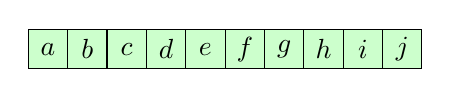
\begin{tikzpicture}
\filldraw[fill=green!20,draw=black] (0,0) rectangle (5,0.5);
\foreach \x in {1,2,...,9} {
  \draw (0.5*\x,0) -- ++(0,0.5);
}
\foreach \x/\t in {0/a,1/b,2/c,3/d,4/e,5/f,6/g,7/h,8/i,9/j} {
  \draw (0.5*\x+0.25,0.25) node {$\t$};
}
\end{tikzpicture}
\caption{Voorstelling van een \dsarray{}}
\end{figure}
%\end{block}
\end{frame}
\subsection{In Java}
\subsubsection{Declaratie}
\begin{frame}[fragile]{\dsarray{} in Java: declaratie}
In Java wordt een \dsarray{} aangemaakt door het type van de elementen te specificeren gevolgd door vierkante haken (\texttt{[]}). Tussen de vierkante haken wordt de lengte geplaatst:
\begin{example}[Declaratie \dsarray{}]
\begin{lstlisting}
int[] rijVanGetallen = new int[5];

int n = 20;
String[] rijVanStrings = new String[n];

int k = 5;
double[] rijVanDoubles = new double[n+k];
\end{lstlisting}
\end{example}
\begin{hint}[Declaratie en toewijzing]
Indien men een array wil initialiseren waarbij de elementen ook al ingevuld worden, kan men gebruik maken van accolades:
\begin{lstlisting}
String[] namen = new String[]{"Samson","Gert","Alberto","Octaaf"};
\end{lstlisting}
\end{hint}
\end{frame}
\begin{frame}[fragile]{\dsarray{} in Java: declaratie: primitief versus klasse}
Java maakt een onderscheid tussen de declaratie van een array van \term{primitieve datatypes} (\dsint{}, \dsfloat{}, \dslong{},...) en \term{klasse-datatypes} (\dsobject{}, \dsstring{}):
\begin{enumerate}
 \item Bij primitieve datatypes wordt de \term{data} in de array opgeslagen.
 \begin{figure}[H]
 \centering
 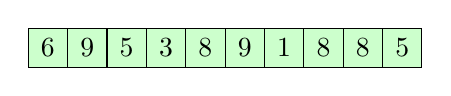
\begin{tikzpicture}
 \tikzarray{10}{6,9,5,3,8,9,1,8,8,5}
 \end{tikzpicture}
 \end{figure}
 \item Bij klasse-datatypes worden \term{pointers} in de array opgeslagen.
 \begin{figure}[H]
 \centering
 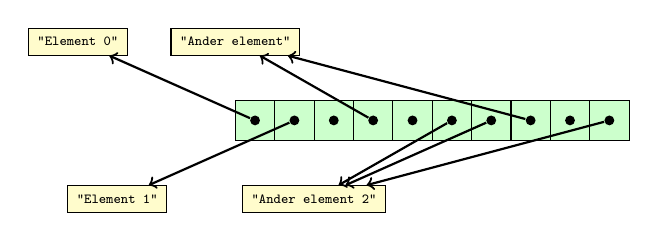
\begin{tikzpicture}
 \tikzarrayptr{10}{paex}
 \begin{scope}[xshift=-2cm,yshift=1 cm]
 \strobj{e0}{Element 0}
 \end{scope}
 \begin{scope}[xshift=-1.5cm,yshift=-1 cm]
 \strobj{e1}{Element 1}
 \end{scope}
 \begin{scope}[xshift=0cm,yshift=1 cm]
 \strobj{e2}{Ander element}
 \end{scope}
 \begin{scope}[xshift=1cm,yshift=-1 cm]
 \strobj{e3}{Ander element 2}
 \end{scope}
 \draw[pointer] (paex1) -- (e0);
 \draw[pointer] (paex2) -- (e1);
 \draw[pointer] (paex4) -- (e2);
 \draw[pointer] (paex6) -- (e3);
 \draw[pointer] (paex7) -- (e3);
 \draw[pointer] (paex8) -- (e2);
 \draw[pointer] (paex10) -- (e3);
 \end{tikzpicture}
 \end{figure}
\end{enumerate}
\end{frame}
\subsubsection{Toegang tot elementen}
\begin{frame}[fragile]{\dsarray{} in Java: toegang tot elementen}
In Java kan men een element in een \dsarray{} opvragen door na de naam van de variabele tussen vierkante haken de index te vermelden. De index telt vanaf 0. Het eerste element staat dus op index 0. Men kan de waarde van een element in een array dan uitlezen en aanpassen.
\begin{example}[Toegang tot elementen van een \dsarray{}]
\begin{lstlisting}
int[] rijVanGetallen = new int[5];

rijVanGetallen[0] = 1;
rijVanGetallen[1] = 1;
rijVanGetallen[2] = rijVanGetallen[0]+1;
rijVanGetallen[3] = 5;
rijVanGetallen[4] = 8;
\end{lstlisting}
\end{example}
\end{frame}
\subsubsection{Lengte}
\begin{frame}[fragile]{\dsarray{} in Java: lengte}
In Java kan men de lengte van een \dsarray{} opvragen door het \texttt{length} argument op te roepen.
\begin{example}[Lengte opvragen van een \dsarray{}]
\begin{lstlisting}
int[] rijVanGetallen = new int[5];
System.out.println(rijVanGetallen.length);
\end{lstlisting}
\end{example}
\end{frame}
\section{ArrayList}
\subsection{Definitie}
\begin{frame}{\dsarraylist{}: definitie}
\begin{definition}[\dsarraylist{}]
Een \term{\dsarraylist{}} is een gegevensstructuur die bestaat uit een opeenvolging van elementen. Elk element in een \dsarraylist{} heeft een unieke \term{index} en is toegankelijk in constante tijd (dit wordt ook wel \term{Random-Access} genoemd). Een \dsarraylist{} heeft een variabele \term{lengte}: we hoeven geen lengte op te geven bij de constructie van een \dsarraylist{} en in principe kunnen we eindeloos elementen toevoegen.
\end{definition}
Visueel zullen we een \dsarraylist{} in deze presentatie voorstellen als een opeenvolging van hokjes, maar met een open einde. Zoals hier:
\begin{figure}
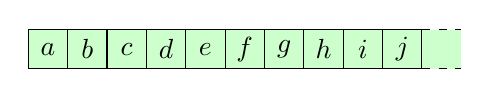
\begin{tikzpicture}
\tikzarraylist{10}{a,b,c,d,e,f,g,h,i,j}
\end{tikzpicture}
\caption{Voorstelling van een \dsarraylist{}}
\end{figure}
\end{frame}
\subsection{In Java}
\subsubsection{Declaratie}
\begin{frame}[fragile]{\dsarraylist{} in Java: declaratie}
Een \dsarraylist{} is een klasse die uit de Java-bibliotheek komt. Deze klasse is \texttt{java.util.ArrayList}. Daarom kunnen we een \dsarraylist{} aanmaken zoals andere objecten. Een \dsarraylist{} is een \term{generische klasse}: we kunnen een type-parameter tussen scheve haken (\texttt{<>}).
\examplecode{Declaratie \dsarraylist{}}{arraylistdeclaration0}
\end{frame}
\begin{frame}[fragile]{\dsarraylist{} in Java: Primitieve types bij generische klasses}
\begin{letop}[Primitieve types bij generische klasses]
\small{Men kan een \dsarraylist{} declareren met elk \term{klasse-type}, primitieve types zijn niet toegelaten! Hiervoor heeft Java schaduwklasses ingevoerd:}
\begin{table}
\centering
\small{\begin{tabular}{l|l}
Primitief type&Klasse-type\\\hline
\texttt{byte}&\texttt{Byte}\\
\texttt{short}&\texttt{Short}\\
\texttt{int}&\texttt{Integer}\\
\texttt{long}&\texttt{Long}\\
\texttt{float}&\texttt{Float}\\
\texttt{double}&\texttt{Double}\\
\texttt{boolean}&\texttt{Boolean}\\
\texttt{char}&\texttt{Char}\\
\end{tabular}}
\caption{Omzetten van primitieve types naar klasse-types}
\end{table}
\end{letop}
\end{frame}
\subsubsection{Toevoegen en verwijderen}
\begin{frame}[fragile]{\dsarraylist{} in Java: toevoegen/verwijderen van elementen}
\dsarraylist{} biedt methodes aan om elementen toe te voegen en te verwijderen:
\small{\begin{itemize}
 \item \texttt{public boolean add (E element)}: voegt een element toe op het einde van de \dsarraylist{}
 \item \texttt{public void add (int index, E element)}: voegt een element toe op plaats \texttt{index}, de overige elementen worden naar rechts opgeschoven
 \item \texttt{public E remove (int index)}: verwijdert het element op \texttt{index}. De elementen erna worden naar links opgeschoven. Het element die oorspronkelijk op deze plaats stond, wordt teruggegeven
 \item \texttt{public boolean remove (Object o)}: het opgegeven element wordt uit de \dsarraylist{} verwijdert. Geeft \texttt{true} terug indien dit element in de \dsarraylist{} aanwezig was.
\end{itemize}}
\end{frame}
\begin{frame}[fragile]{\dsarraylist{} in Java: \texttt{add (E element)}}
\begin{methodexample}[\texttt{add (E element)}]
\begin{center}
\begin{animateinline}{1}
\methodexec{arraylistadd0me}{1}{}{
}\newframe

\methodexec{arraylistadd0me}{2}{namen}{
\begin{scope}[xshift=7 cm]
\tikzarraylistptr{0}{namenlist}
\pointleftbridge{ptrnamen}{offsetnamenlist}
\end{scope}
}\newframe
\methodexec{arraylistadd0me}{3}{namen}{
\begin{scope}[xshift=3 cm,yshift=1 cm]
\strobj{elem0}{Samson}
\end{scope}
\begin{scope}[xshift=7 cm]
\tikzarraylistptr{1}{namenlist}
\pointleftbridge{ptrnamen}{offsetnamenlist}
\pointarraytopright{namenlist1}{elem0}
\end{scope}
}\newframe

\methodexec{arraylistadd0me}{4}{namen}{
\begin{scope}[xshift=3 cm,yshift=1 cm]
\strobj{elem0}{Samson}
\end{scope}
\begin{scope}[xshift=4 cm,yshift=-0.5 cm]
\strobj{elem1}{Gert}
\end{scope}
\begin{scope}[xshift=7 cm]
\tikzarraylistptr{2}{namenlist}
\pointleftbridge{ptrnamen}{offsetnamenlist}
\pointarraytopright{namenlist1}{elem0}
\pointarraybotright{namenlist2}{elem1}
\end{scope}
}\newframe

\methodexec{arraylistadd0me}{5}{namen}{
\begin{scope}[xshift=3 cm,yshift=1 cm]
\strobj{elem0}{Samson}
\end{scope}
\begin{scope}[xshift=4 cm,yshift=-0.5 cm]
\strobj{elem1}{Gert}
\end{scope}
\begin{scope}[xshift=5 cm,yshift=1.5 cm]
\strobj{elem2}{Octaaf}
\end{scope}
\begin{scope}[xshift=7 cm]
\tikzarraylistptr{3}{namenlist}
\pointleftbridge{ptrnamen}{offsetnamenlist}
\pointarraytopright{namenlist1}{elem0}
\pointarraybotright{namenlist2}{elem1}
\pointarraytopright{namenlist3}{elem2}
\end{scope}
}
\end{animateinline}
\end{center}
\end{methodexample}
\end{frame}
\begin{frame}[fragile]{\dsarraylist{} in Java: \texttt{add (int index, E element)}}
\begin{methodexample}[\texttt{add (int index, E element)}]
\begin{center}
\begin{animateinline}{1}
\methodexec{arraylistadd1me}{5}{namen}{
\begin{scope}[xshift=3 cm,yshift=1 cm]
\strobj{elem0}{Samson}
\end{scope}
\begin{scope}[xshift=4 cm,yshift=-0.5 cm]
\strobj{elem1}{Gert}
\end{scope}
\begin{scope}[xshift=5 cm,yshift=1.5 cm]
\strobj{elem2}{Octaaf}
\end{scope}
\begin{scope}[xshift=7 cm]
\tikzarraylistptr{3}{namenlist}
\pointleftbridge{ptrnamen}{offsetnamenlist}
\pointarraytopright{namenlist1}{elem0}
\pointarraybotright{namenlist2}{elem1}
\pointarraytopright{namenlist3}{elem2}
\end{scope}
}\newframe

\methodexec{arraylistadd1me}{6}{namen}{
\begin{scope}[xshift=3 cm,yshift=1 cm]
\strobj{elem0}{Samson}
\end{scope}
\begin{scope}[xshift=4 cm,yshift=-0.5 cm]
\strobj{elem1}{Gert}
\end{scope}
\begin{scope}[xshift=5 cm,yshift=1.5 cm]
\strobj{elem2}{Octaaf}
\end{scope}
\begin{scope}[xshift=6 cm,yshift=-1 cm]
\strobj{elem3}{Alberto}
\end{scope}
\begin{scope}[xshift=7 cm]
\tikzarraylistptr{4}{namenlist}
\pointleftbridge{ptrnamen}{offsetnamenlist}
\pointarraytopright{namenlist1}{elem0}
\pointarraybotright{namenlist2}{elem1}
\pointarraytopright{namenlist4}{elem2}
\pointarraybotright{namenlist3}{elem3}
\end{scope}
}
\end{animateinline}
\end{center}
\end{methodexample}
\end{frame}
\begin{frame}[fragile]{\dsarraylist{} in Java: \texttt{remove (int index)}}
\begin{methodexample}[\texttt{remove (int index)}]
\begin{center}
\begin{animateinline}{1}
\methodexec{arraylistremove0me}{6}{namen}{
\begin{scope}[xshift=3 cm,yshift=1 cm]
\strobj{elem0}{Samson}
\end{scope}
\begin{scope}[xshift=4 cm,yshift=-0.5 cm]
\strobj{elem1}{Gert}
\end{scope}
\begin{scope}[xshift=5 cm,yshift=1.5 cm]
\strobj{elem2}{Octaaf}
\end{scope}
\begin{scope}[xshift=6 cm,yshift=-1 cm]
\strobj{elem3}{Alberto}
\end{scope}
\begin{scope}[xshift=7 cm]
\tikzarraylistptr{4}{namenlist}
\pointleftbridge{ptrnamen}{offsetnamenlist}
\pointarraytopright{namenlist1}{elem0}
\pointarraybotright{namenlist2}{elem1}
\pointarraytopright{namenlist4}{elem2}
\pointarraybotright{namenlist3}{elem3}
\end{scope}
}\newframe

\methodexec{arraylistremove0me}{7}{namen,verw}{
\begin{scope}[xshift=3 cm,yshift=1 cm]
\strobj{elem0}{Samson}
\end{scope}
\begin{scope}[xshift=4 cm,yshift=-0.5 cm]
\strobj{elem1}{Gert}
\end{scope}
\begin{scope}[xshift=5 cm,yshift=1.5 cm]
\strobj{elem2}{Octaaf}
\end{scope}
\begin{scope}[xshift=6 cm,yshift=-1 cm]
\strobj{elem3}{Alberto}
\end{scope}
\begin{scope}[xshift=7 cm]
\tikzarraylistptr{3}{namenlist}
\pointleftbridge{ptrnamen}{offsetnamenlist}
\pointarraytopright{namenlist1}{elem0}
\pointarraytopright{namenlist3}{elem2}
\pointarraybotright{namenlist2}{elem3}
\pointlertbridge{ptrverw}{elem1}
\end{scope}
}\newframe

\methodexec{arraylistremove0me}{8}{namen,verw}{
\begin{scope}[xshift=3 cm,yshift=1 cm]
\strobj{elem0}{Samson}
\end{scope}
% \begin{scope}[xshift=4 cm,yshift=-0.5 cm]
% \strobj{elem1}{Gert}
% \end{scope}
\begin{scope}[xshift=5 cm,yshift=1.5 cm]
\strobj{elem2}{Octaaf}
\end{scope}
\begin{scope}[xshift=6 cm,yshift=-1 cm]
\strobj{elem3}{Alberto}
\end{scope}
\begin{scope}[xshift=7 cm]
\tikzarraylistptr{2}{namenlist}
\pointleftbridge{ptrnamen}{offsetnamenlist}
\pointarraytopright{namenlist1}{elem0}
\pointarraybotright{namenlist2}{elem3}
\pointlertbridge{ptrverw}{elem2}
\end{scope}
}
\end{animateinline}
\end{center}
\end{methodexample}
\end{frame}
\begin{frame}[fragile]{\dsarraylist{} in Java: \texttt{remove (Object o)}}
\begin{methodexample}[\texttt{remove (Object o)}]
\begin{center}
\begin{animateinline}{1}
\methodexec{arraylistremove1me}{8}{namen,verw}{
\begin{scope}[xshift=3 cm,yshift=1 cm]
\strobj{elem0}{Samson}
\end{scope}
% \begin{scope}[xshift=4 cm,yshift=-0.5 cm]
% \strobj{elem1}{Gert}
% \end{scope}
\begin{scope}[xshift=5 cm,yshift=1.5 cm]
\strobj{elem2}{Octaaf}
\end{scope}
\begin{scope}[xshift=6 cm,yshift=-1 cm]
\strobj{elem3}{Alberto}
\end{scope}
\begin{scope}[xshift=7 cm]
\tikzarraylistptr{2}{namenlist}
\pointleftbridge{ptrnamen}{offsetnamenlist}
\pointarraytopright{namenlist1}{elem0}
\pointarraybotright{namenlist2}{elem3}
\pointlertbridge{ptrverw}{elem2}
\end{scope}
}\newframe

\methodexec{arraylistremove1me}{9}{namen,verw,wasin/false}{
\begin{scope}[xshift=3 cm,yshift=1 cm]
\strobj{elem0}{Samson}
\end{scope}
% \begin{scope}[xshift=4 cm,yshift=-0.5 cm]
% \strobj{elem1}{Gert}
% \end{scope}
\begin{scope}[xshift=5 cm,yshift=1.5 cm]
\strobj{elem2}{Octaaf}
\end{scope}
\begin{scope}[xshift=6 cm,yshift=-1 cm]
\strobj{elem3}{Alberto}
\end{scope}
\begin{scope}[xshift=7 cm]
\tikzarraylistptr{2}{namenlist}
\pointleftbridge{ptrnamen}{offsetnamenlist}
\pointarraytopright{namenlist1}{elem0}
\pointarraybotright{namenlist2}{elem3}
\pointlertbridge{ptrverw}{elem2}
\end{scope}
}\newframe

\methodexec{arraylistremove1me}{10}{namen,verw,wasin/true}{
\begin{scope}[xshift=3 cm,yshift=1 cm]
\strobj{elem0}{Samson}
\end{scope}
% \begin{scope}[xshift=4 cm,yshift=-0.5 cm]
% \strobj{elem1}{Gert}
% \end{scope}
\begin{scope}[xshift=5 cm,yshift=1.5 cm]
\strobj{elem2}{Octaaf}
\end{scope}
% \begin{scope}[xshift=6 cm,yshift=-1 cm]
% \strobj{elem3}{Alberto}
% \end{scope}
\begin{scope}[xshift=7 cm]
\tikzarraylistptr{1}{namenlist}
\pointleftbridge{ptrnamen}{offsetnamenlist}
\pointarraytopright{namenlist1}{elem0}
%\pointarraybotright{namenlist2}{elem3}
\pointlertbridge{ptrverw}{elem2}
\end{scope}
}
\end{animateinline}
\end{center}
\end{methodexample}
\end{frame}
% \subsubsection{Toegang tot elementen}
% \begin{frame}[fragile]{\dsarraylist{} in Java: toegang tot elementen}
% Omdat \dsarraylist{} een gewone klasse is, krijgt met toegang tot de elementen via methodes:
% \begin{itemize}
%  \item \texttt{public E get (int index)}
%  \item \texttt{public E set (int index, E element)}
% \end{itemize}
% \end{frame}
% \subsection{Lengte}
% \begin{frame}[fragile]{\dsarraylist{} in Java: lengte (aantal elementen)}
% We kunnen het aantal elementen in de \dsarraylist{} opvragen met behulp van de \texttt{size()}-methode.
% \begin{example}[Lengte van een \dsarraylist{}]
% \begin{lstlisting}
% ArrayList<String> namen = new ArrayList<String>();
% namen.add("Samson");
% namen.add("Gert");
% namen.add("Alberto");
% namen.add("Octaaf");
% System.out.println(namen.size()); //4
% \end{lstlisting}
% \end{example}
% \begin{letop}[\texttt{length} versus \texttt{size()}]
% Bij een \dsarray{} vragen we de lengte op met behulp van \texttt{.length}. Bij een \dsarraylist{} is dat met de \texttt{size()}-methode. Omgekeerd werkt dit niet!
% \end{letop}
% \end{frame}
% \subsubsection{Andere operaties}
%\section{LinkedList}
\subsection{Definitie}
\begin{frame}{\dslinkedlist{}: definitie}
\begin{definition}[\dslinkedlist{}]

\end{definition}
\end{frame}
\subsection{In Java}
\subsubsection{Declaratie}
\subsubsection{Toegang tot elementen}
\subsubsection{Toevoegen en verwijderen}
\subsubsection{Andere operaties}
\subsection{Werking}
\subsection{Implementatie}
%\section{Interface}
\begin{frame}[fragile]{Interface}
\begin{definition}[Interface]
Een interface is een lijst van methodes die klasses die de interface implementeren moeten aanbieden.
\end{definition}
\begin{example}[\texttt{Praat}-interface]
\begin{lstlisting}
public interface Praat {

  void praat ();

}
\end{lstlisting}
\end{example}
\end{frame}
\subsection{Implementeren}
\begin{frame}[fragile]{Implementeren van een Interface}
Alle klasses die de interface \term{implementeren}, moeten de methodes invullen:
\begin{example}[Gert-klasse]
\begin{lstlisting}
public class Gert implements Praat {

  public void praat () {
    System.out.println("Hallo, mijn naam is Gert.");
  }

}
\end{lstlisting}
\end{example}
\begin{example}[Samson-klasse]
\small{\begin{lstlisting}
public class Samson implements Praat {

  public void praat () {
    System.out.println("Mwoa en ik ben Samson.");
  }

}
\end{lstlisting}}
\end{example}
\end{frame}
\end{document}